\section{\arch for Hypervisor Replacement}
In this section, we introduce the design and implementation of \arch for 
live hypervisor replacement, followed by live OS replacement 
in the next section. 
The key idea behind \arch is as follows: Instead of copying the memory 
of VMs from the stale hypervisor to the co-located replacement hypervisor, 
\arch transfers the ownership of VMs' physical memory pages via page table remapping. 
Such memory ownership relocation is fast and leads to sub-10ms live hypervisor 
replacement. In addition, \arch includes optimizations to further mitigate 
nesting overhead during normal execution of VMs.
We first introduce memory translation under nested virtualization, 
followed by hyperplexor-based hypervisor switching, and finally 
optimizations to mitigate nesting overheads.


%The key design goals of the proposed work are transparency and minimum 
%service disruption in guests. The architecture of live hypervisor replacement
%is shown in Figure~\ref{fig:arch}. Using nested virtualization, the hypervisors at L1 and unmodified guests are run on thin hyperplexor at L0. Using SR-IOV, a single PCI device or physical function is presented as multiple virtual functions to hypervisors to reduce the performance overhead in guest due to nested virtualization. Upon a migration event, an updated hypervisor is first started on thin hyperplexor. The updated hypervisor then replaces the aged hypervisor by co-mapping the memory of guest. The hyperplexor transfers the memory mappings using grant table mechanism where the  guest page frames are mapped to the updated hypervisor followed by unmapping of memory from the aged hypervisor. The completion of hypervisor replacement is marked by pausing the guest and transferring the vCPU and I/O states to the updated hypervisor.  

\begin{figure}[t!]
 	  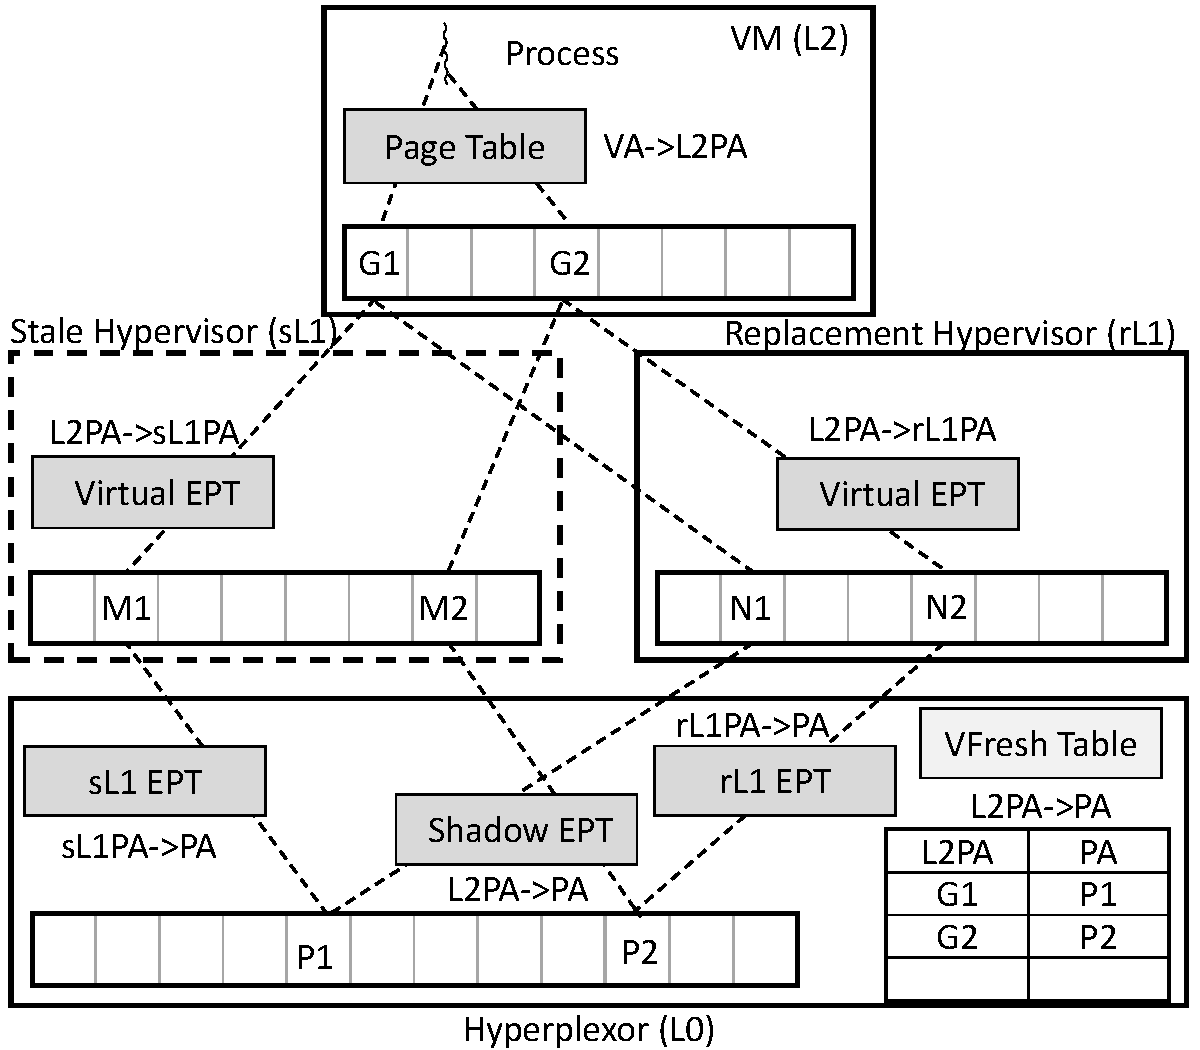
\includegraphics[width=0.45\textwidth]{figures/vfresh-table.pdf}
  \caption{Memory translations for hypervisor replacement.}
  \label{fig:mapping}
  %\includegraphics[width=15cm,height=6cm,keepaspectratio]{architecture__1_.jpg}
\end{figure}

\subsection{Memory Translation for Nested Virtualization}
In native execution mode (without virtualization), a page table stores the mappings between 
the virtual addresses (VA) of a process to its physical addresses (PA) 
where memory content actually resides. When a VA is accessed by 
a process, the hardware memory management unit (MMU) uses the page table 
to translate the VA to its PA.

In single-level virtualization, an additional level of address translation 
is added by the hypervisor for virtualizing the memory translations for VMs. 
The page table of a process running on a VM stores the mappings from the guest 
virtual addresses (GVA) of a process to the guest physical addresses (GPA),
which is the virtualized view of memory seen by the VM. 
The hypervisor uses another page table, called the extended page table (EPT) 
to map GPA to its physical addresses (PA). 
As with traditional page tables, an EPT is constructed incrementally upon page faults.
As a VM tries to access previously unallocated GPA, EPT violations are generated, 
like page faults for a process. 
These faults are processed by the hypervisor which allocates a new physical page 
for the faulting GPA. 

In nested virtualization, as shown in \fref{fig:mapping}, 
three levels of translations are needed. A process's virtual address is translated to the GPA 
of the layer-2 VM (labeled L2PA). 
An L2PA is translated to the guest physical address of the L1 hypervisor (L1PA) using a
{\em virtual EPT} for the layer-2 VM maintained by the L1 hypervisor. Finally, 
the L1PA is translated to the physical address of the host (PA) using the L1 hypervisor's EPT  
maintained by the hyperplexor at L0. Since, the MMU can translate only two levels 
of memory mappings, the hyperplexor at L0 combines the virtual EPT at L1 and the EPT at L0 to 
construct a {\em Shadow EPT} for every L2 VM.
The MMU uses the process page table in the L2 VM and the shadow EPT at L0 to translate a 
process VA to its PA. The shadow EPT is updated whenever the corresponding virtual EPT in L1 
and/or the EPT in L0 are updated.
 
\subsection{Hypervisor Replacement Overview}
We now present an overview of the hypervisor replacement mechanism followed by  low-level details.
Consider a VM that initially runs on the stale L1 hypervisor which in turn runs on the 
thin L0 hyperplexor.
To replace the stale hypervisor, the hyperplexor creates a new replacement L1 hypervisor (with pre-installed updates) 
and transfers the ownership of all L2 VMs' physical pages to this replacement hypervisor.

The page mappings from an L2 VM's guest physical address (L2PA) to the physical memory (PA) are
available in the shadow EPT of the L2 VM. 
Ideally, the hyperplexor could accomplish the L2 VM's relocation
simply by reusing the shadow EPT, albeit under the replacement hypervisor's control.
However, since the shadow EPT is the result of combining a nested
VM's virtual EPT in L1 and L1's own EPT in L0, these two intermediate mappings 
must be accurately reconstructed in the new address translation path via 
the replacement hypervisor. 

To accomplish this reconstruction, the replacement hypervisor must coordinate 
with the hyperplexor.
It does so by preparing a skeletal L2 VM to receive each incoming L2 VM
and reserves unallocated L1 page frame numbers in its guest-physical address space (L1PA) 
where the incoming VM's pages will be mapped. 
The replacement hypervisor then communicates the identity of these reserved page frames 
in L1PA to the hyperplexor (via a hypercall), so that the hyperplexor
can map these reserved page frames to the incoming L2 VM's existing physical pages.
Note that the reserved L1 page frames in the replacement hypervisor may not be the same as 
that in stale hypervisor as shown in \fref{fig:mapping}. 

The transfer of execution control is then  performed as follows.
The L2 VM's execution is paused at the stale hypervisor
and its execution state (consisting of all VCPU and I/O states) 
are transferred to the replacement hypervisor's control, which then resumes execution 
of the L2 VM. This switch over operation can be accomplished quickly 
(sub-10ms in our prototype) since no memory content is copied during this step.
Finally, once the control of the L2 VM is transferred to the replacement hypervisor, 
the stale hypervisor can unmap the L2 VM's  memory from its address space and be safely deprovisioned. 

As the relocated L2 VM begins execution on the replacement hypervisor,
it generates page faults against its memory accesses.
The entries in the new intermediate mapping tables (the virtual EPT and replacement hypervisor's 
L1 EPT) are populated on-demand to reflect the original physical 
pages used by the L2 VM under the stale hypervisor. 
In other words, the shadow EPT reconstructed for the relocated
VM ends up being identical to its erstwhile shadow EPT used under the stale hypervisor, while 
the new intermediate mapping tables are correspondingly adjusted.
We nest describe low-level details of \arch implementation.



\subsection{Implementation Details} 
We developed a prototype of \arch using the KVM/QEMU virtualization platforms with Linux kernel 
version 4.13.0 and QEMU version 2.9.0. KVM is a linux kernel module which is responsible for 
core hypervisor functionalities. QEMU is a user space process that manages VM control operations,
including live migration, and emulates its I/O operations. The VM runs unmodified Linux kernel 
version 4.13.0 and uses para-virtual I/O devices.
Our hypervisor replacement solution was implemented by modifying QEMU's live migration mechanism, besides
modifications to KVM to implement page remappings described above. 

Different from QEMU's live migration, 
\arch's hypervisor replacement operation only involves the transfer of VCPU and I/O state of the VM. 
Since the relocation of L2 VM's memory pages is performed 
out of the critical path of hypervisor replacement, we modified QEMU's live migration
to disable dirty page tracking, transfer of page contents via pre-copy iterations, and
also the transfer of residual dirty pages during the stop-and-copy phase of live migration. 
The VCPUs are paused only during the stop-and-copy phase which results in very low hypervisor 
replacement time.

\subsubsection{The \arch Table}
In KVM's current implementation, the L2 VM's shadow EPT cannot be easily transferred 
from the stale hypervisor to the replacement hypervisor.
Hence, our hyperplexor implementation constructs a parallel table, which we call the {\em \arch table},
to store a copy of the L2-to-physical page mapping information contained in the shadow EPT.
This \arch table is used for reconstructing the same L2PA-to-PA page mappings for 
the relocated VM upon EPT violations.

To construct the \arch table, the hyperplexor needs a list of L2-to-L1 page mappings 
of the VM from the stale hypervisor, using the virtual EPT table. 
% as listed in Table \ref{tab:api}. 
The stale hypervisor invokes a \texttt{hypercall\_put} hypercall multiple times
to pass a complete list of L2-to-L1 page mappings 
of the VM to the hyperplexor. For each received L2-to-L1 page mapping, the hyperplexor translates 
the L1 page number to the physical  page number using the EPT table at L0, and inserts 
the corresponding L2-to-physical page mapping into the {\em \arch table}. 

To relocate the ownership of a L2 VM's memory to the replacement hypervisor, the hyperplexor
needs  the list of L2-to-L1 page mappings of the newly created skeletal VM from the replacement hypervisor.
The replacement hypervisor invokes another \texttt{hypercall\_map} hypercall multiple times
to pass these mappings to the hyperplexor. For each received L2-to-L1 page mapping, the hyperplexor 
(1) looks up the {\em \arch table} to find the L2-to-PA mapping with the L2 page number 
as the key; and (2) installs the L1-to-PA page mapping in the replacement hypervisor's 
EPT table. More specifically, \arch translates each L1 guest frame number to its  host virtual address (HVA), 
installs the HVA-to-PA page mapping in the page table of the VM's QEMU process, and at last invalidates the 
corresponding entry in the EPT table, which is reconstructed later upon an EPT  fault.
Also, to clear any pre-existing GFN mappings of the replacement hypervisor, the hyperplexor flushes 
the entries in TLB and page table of QEMU, before resuming the relocated VM.

%TODO: Kartik: Spoorti, The following details can be included in your dissertation. Its too low for the paper.
%\para{Memory Relocation:}
%The source VM's QEMU makes an IOCTL to request current KVM hypervisor to pin the VM pages in memory during the boot time. Hypervisor uses memory slots to get the VM frame numbers (GFNs) of the VM and translates all the VM GFNs to hypervisor GFNs. KVM then transfers the VM GFNs and hypervisor GFNs mapping information to the hyperplexor using \texttt{hypercall\_set} hypercalls. The hyperplexor pins the pages in memory using the hypervisor GFNs. Hyperplexor creates the \arch table with VM GFN to physical frame number (PFNs) mappings and uses a VM ID to indicate the owner of the \arch table. 
%
%When the current hypervisor has to be replaced with updated hypervisor, the destination VM makes an IOCTL to the new KVM hypervisor to map the VM pages to the PFNs of the source VM using the \arch table. The new hypervisor also iterates through the memory slots to get all the VM GFNs. KVM then gets the free hypervisor GFNs to map the VM GFNs. To ensure that the hypervisor GFNs are clear of any previous mappings, we flush the entries in TLB and page table of QEMU. The VM GFNs and hypervisor GFNs are transferred to hyperplexor through \texttt{hypercall\_map} hypercalls. The hyperplexor maps the destination VM GFNs to the PFNs using the \arch table and adds the destination VM to the owner of the \arch table..
%
%A hypercall is costly as it involves a switch from the non-root mode to the root mode with a VMExit. For each VMExit, the hypervisor has to store the VMExit information, save the state of the VM and load the host state information (vice-versa on VMEntry). To minimize the number of hypercalls, we write the VM GFN to hypervisor GFN mappings to pages allocated in hypervisor and transfer the address of the pages to the hyperplexor. The number of hypercalls reduce to the number of pages required to store the memory mappings information. The \arch table is implemented as a hash table for fast lookup of the VM GFN to PFN mapping.


%\begin{figure}[t!]
%  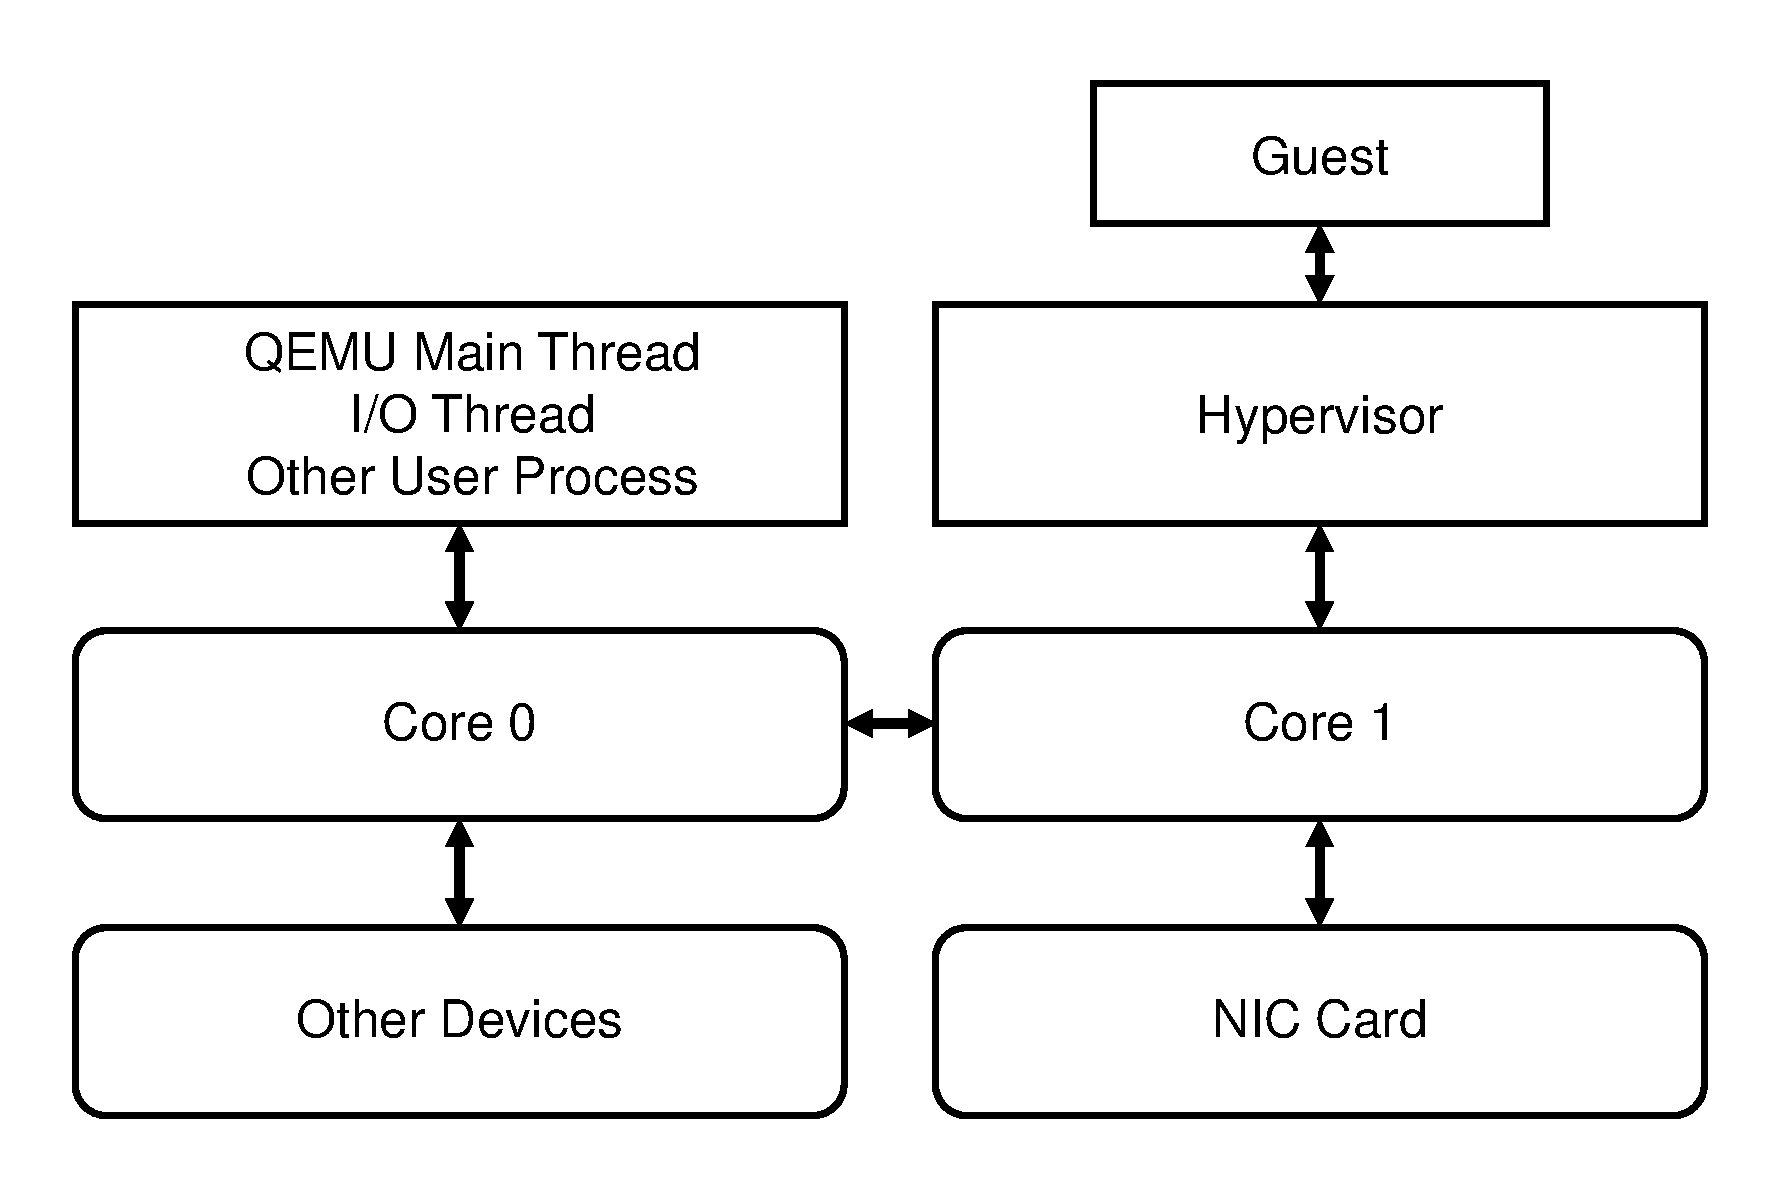
\includegraphics[width=0.4\textwidth]{figures/nested_virtualization_overhead_setup.pdf}
%  \caption{Optimizations to reduce overhead of nested virtualization: dedicated and isolated CPUs with Posted Interrupt support and halt\_poll\_ns disabled.}
%  \label{fig:optimizations}
  %\includegraphics[width=15cm,height=6cm,keepaspectratio]{architecture__1_.jpg}
%\end{figure}

\subsubsection{Mitigating Nesting Overheads}
\label{sec:overhead}
In comparison with the traditional single-level virtualization 
setup, where the hypervisor directly controls the hardware,
nested virtualization can introduce additional emulation overheads, especially for I/O virtualization. To mitigate such overhead, \arch uses the direct device assignment of network interface cards (NIC) to the hypervisor. 

%\textbf{Background}
Existing virtualization techniques (e.g., KVM \cite{kivity2007kvm}) support the full virtualization mode through device emulation \cite{sugerman2001virtualizing} and para-virtualization using virtio drivers \cite{russell2008virtio, barham2003xen}  in VMs. 
%They also support direct device assignment  to the guest \cite{ben2006utilizing}. 
For example, QEMU \cite{bellard2005qemu} emulates I/O devices requiring no modifications to VMs. When VMs access the devices, the I/O instructions are trapped into hypervisor leading to a number of VM/host context switches, resulting in lower performance of VMs. The para-virtualized devices offer better performance compared to device emulation, as the modified drivers in VMs avoid excessive VM/host switches for the I/O workloads. With Intel's VT-d \cite{abramson2006intel}, direct device assignment offers improved performance, as VMs directly interact with the devices bypassing the hypervisor.    
%With hardware virtualization technology, 
Further, SR-IOV \cite{dong2008sr} enables a single network device to present itself as multiple virtual NICs to VMs through virtual functions (VFs). Using a VF, a VM directly interacts with the network device --- with Intel's hardware support, VMs can directly access device memory through IOMMU which converts VMs physical addresses to host physical addresses.

%\textbf{Direct Device Assignment of Network Interface Card}
In this paper, \arch uses VFs to achieve network performance in nested guest to match the performance of a single-level guest and minimize the CPU Utilization in hyperplexor. VFIO \cite{vfiodriver} driver supports direct device assignment to a virtual machine. As shown in \fref{fig:vFresharch} every hypervisor running on hyperplexor is assigned one virtual function. The guest running on hypervisor uses para-virtualized driver to run the I/O workloads. \arch further applies many optimizations to provide hypervisor with enough resources and reduce the CPU utilization on hyperplexor. The goal is to run the hypervisor with minimum hyperplexor intervention. We describe the optimization techniques in detail in the following sections.

\begin{figure}[t!]
 	  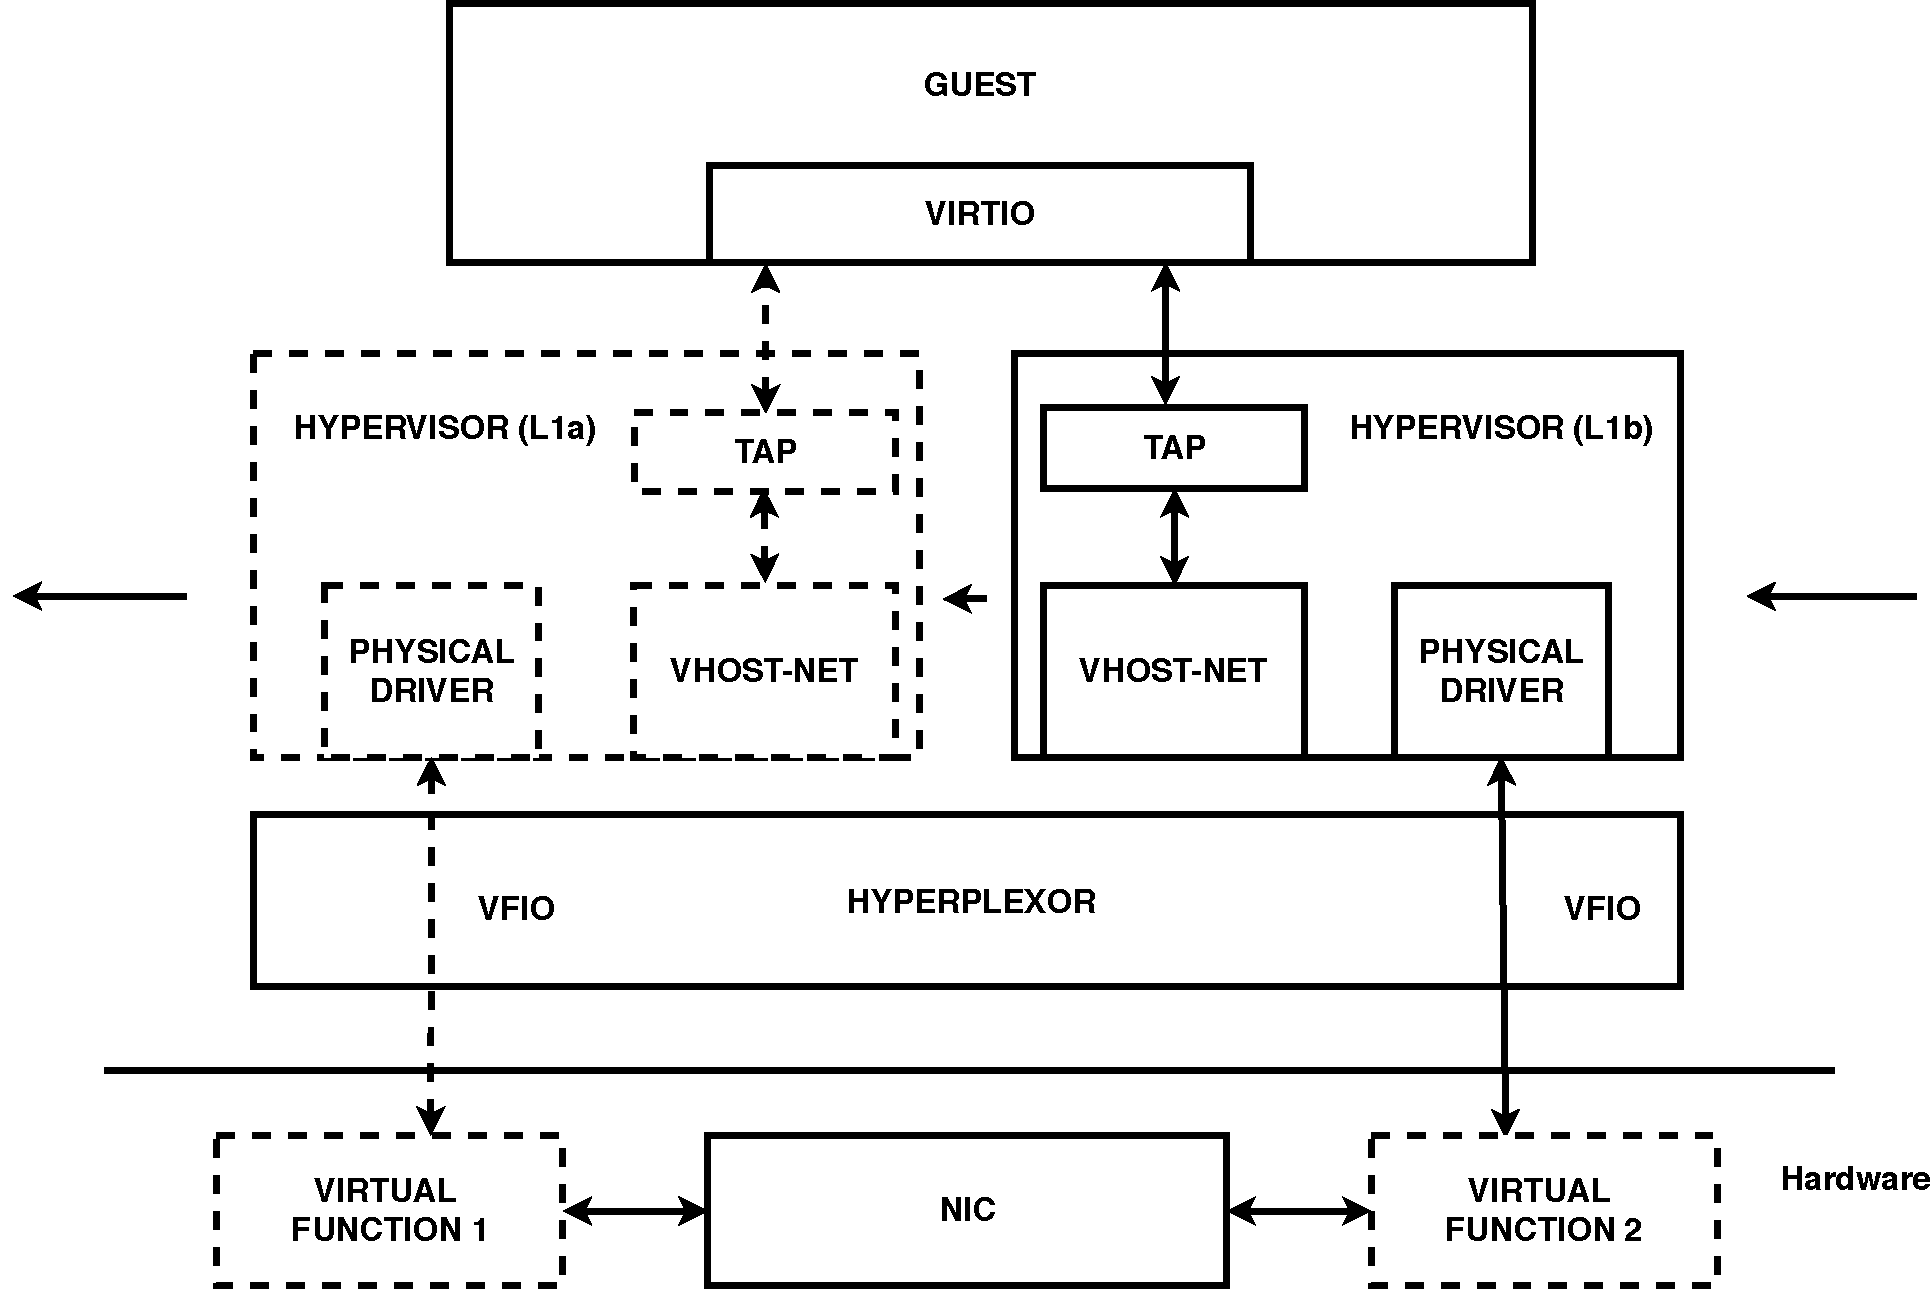
\includegraphics[width=0.45\textwidth]{figures/architecture_modified.pdf}
  \caption{Architecture for hypervisor replacement with direct-device assignment and thin hyperplexor.}
%TODO: Please fix this caption
  \label{fig:vFresharch}
  \vspace{0.2in}
  %\includegraphics[width=15cm,height=6cm,keepaspectratio]{architecture__1_.jpg}
\end{figure}

%\begin{itemize}
%\item \textbf{\textit{Reducing Memory Footprint of Hyperplexor}}
\para{Memory Footprint:}
As the hyperplexor involvement is minimal, it is configured with essential packages, device drivers and services reducing the memory consumption. The size of the hyperplexor without VM is 90 MB of the available memory compared to the Ubuntu server size 154 MB. The userspace processes and services that where not necessary to run the L1 hypervisor with direct-device assignment were identified and removed. The Linux kernel 4.13.0 is compiled with 32 kernel modules compared to 120 kernel modules in Ubuntu server. 
    
%	\item \textbf{\textit{HLT Exits}}
%halt_poll_ns is a kvm kernel module parameter. When guest VCPU has no work to do or goes idle, the VCPU goes to sleep by executing HLT instruction which causes a VM Exit. The parameter halt_poll_ns specifies how much time the VCPU needs to poll before executing the HLT instructions. This polling interval helps in making the guest more responsive for workloads like the network.

\para{HLT Exits:}
Although a directly assigned network device to a VM gives better performance, the CPU utilization on the host is high due to the idle polling of VCPUs. When the VM is idle, QEMU halts the idle VCPUs by executing a HLT instruction which triggers a VM exit. When the work is available for the VCPU, it has to be woken up to execute the new work. This transition from idle to ready state is costly as it involves context switch and hinders the performance of the VM. To avoid too many transitions, before executing the HLT instruction the VCPU polls for the specified amount of time to check if there is any additional work to be executed. This idle polling of VCPUs reduces the number of VM exits but increases CPU utilization on host. To reduce CPU utilization on host, we disable polling of VCPUs before executing HLT instruction. 
KVM provides a \texttt{halt\_poll\_ns} kernel module parameter to set the value of \texttt{halt\_poll\_ns}. To disable polling we set \texttt{halt\_poll\_ns} to zero. In this paper, as we assign the network device to the hypervisor, we disable the halt polling of hypervisor VCPUs to reduce the CPU Utilization in hyperplexor.
    
   %\item \textbf{\textit{Posted Interrupts}}
\para{Posted Interrupts:}
     When an external interrupt arrives, the CPU switches from non-root mode to root mode (VM Exit) and transfers the control to the hypervisor. Increase in number of external interrupts causes increase in VM Exits. With Intel's VT-d posted interrupt support the external interrupts are delivered to guest without hypervisor intervention. With posted interrupts support the hypervisor can inject a virtual interrupt to guest by updating the fields in the VMCS in guest or non-root mode. Hypervisor notifies the arrival of posted interrupt to the guest by setting the fields Posted Interrupt Request (PIR), Notification Vector (NV) and Outstanding Notification (ON) in Posted Interrupt Descriptor structure. The PIR field is 256 bit long and provides storage for posting the interrupts. The NV field is used to notify the interrupt vector to the guest. The ON bit indicates the processing status of the posted interrupt. We enable posted interrupt feature on the hyperplexor and deliver external interrupts directly to hypervisor without causing exits to hyperplexor.  
     
%\item \textbf{\textit{Dedicated Cores}}
\para{Dedicated Cores:}
All the system processes are running on two cores except the VCPUs which run on dedicated cores. The remaining CPUs are isolated and each VCPU is pinned to one CPU to avoid other processes from contending with VCPUs. 
%As shown in Figure~\ref{fig:optimizations}. 
The QEMU process along with other hyperplexor processes are pinned to CPU0 \& CPU1, and the hypervisor VCPUs run on the dedicated cores. 

%------OLD Stuff----------------------------------------
% \begin{table*}[!htb]
%\small
%  \begin{tabular}{|c|l|l|l|}
%   \hline
%  \arch API & \multicolumn{1}{c|}{Input Parameters} & \multicolumn{1}{c|}{Return Value} & \multicolumn{1}{c|}{Description}\\
%  \hline
%  \hline
%  hypercall\_set &unsigned long base\_addr\_of\_l2gfn\_list, &0 on success,  & Given the VM on the stale hypervisor, \\ 
%  &unsigned long base\_addr\_of\_l1gfn\_list, &failure code otherwise & pass a list of L2-to-L1 page mappings to hyperplexor  \\
%  &unsigned int count, & & for setting up \arch table entries  \\
%  &unsigned int vmid & & storing the L2-to-PA page mappings\\
%  \hline
%
%  hypercall\_map &unsigned long base\_addr\_of\_l2gfn\_list, &0 on success, & Given the VM on the replacement hypervisor, \\
%  &unsigned long base\_addr\_of\_l1gfn\_list, &failure code otherwise & pass a list of L2-to-L1 page mappings to hyperplexor \\
%  &unsigned int count, & & to look up \arch table  \\
%  &unsigned int vmid && for creating L2-to-PA mappings\\
%  \hline
%  
%    hypercall\_set &unsigned long base\_addr\_of\_gva\_list, &0 on success,  & Given a process on the stale OS, \\ 
%  &unsigned long base\_addr\_of\_gfn\_list, &failure code otherwise & pass a list of process-to-VM page mappings   \\
%  &unsigned int count, & & to hypervisor for setting up \arch table entries  \\
%  &unsigned int pid & & storing the GVA-to-PA page mappings\\
%  \hline
%
%  hypercall\_map &unsigned long base\_addr\_of\_gva\_list, &0 on success, & Given the process on the replacement hypervisor, \\
%  &unsigned long base\_addr\_of\_gfn\_list, &failure code otherwise & pass a list of process-to-VM page mappings\\
%  &unsigned int count, & & to look up \arch table  \\
%  &unsigned int pid && to hypervisor for creating GVA-to-PA page mappings\\
%  \hline
%\end{tabular}
%\caption{\arch API}
%\vspace{-0.2in}
%\label{tab:api}
%\end{table*}

%In our approach, we leverage grant table mechanism to transfer the mappings of guest from current hypervisor to updated hypervisor. The current hypervisor requests the hyperplexor to create grant entries in grant table. The updated hypervisor then requests the hyperplexor to map the guest page frame to physical page frames. 

%\textbf{\textit{Background}}
%In Xen, Virtual Machine Monitor (VMM) runs at the highest privilege level which coordinates with host domain (Dom0) or host OS to maintain isolation between guest domains (DomU) or guest OS. Xen supports both full-virtualization and para-virtualization modes. Para-virtualization mode is more efficient with lower virtualization overhead. However, it comes with a trade-off of modifying the guest OS.

%In Xen, the devices are managed by native device drivers run in isolated driver domain (IDD). The network device is presented as a virtual network device to a guest OS. The guest OS runs the front-end driver which shares a device ring buffer with the back-end driver in IDD or Dom0. In para-virtualization mode, a grant table\cite{Pratt05xen3.0} is used as a communication channel between domains. Each domain has a grant table and it is used to share or transfer the memory mappings between the domains. A grant table data structure is shared between Xen and the domain. The grant table entries are indexed using an integer field called grant reference. The reference field indicates which grantee can share the pages with the granter. 

%To share the pages, the granting domain advertises the page to be shared with other domains. The granting domain shares the grant reference ID with the receiving domain. The receiving domain maps the page by updating it's grant table entry. After the receiving domain has finished the operation on the page, the granting domain revokes the access to the page. For page transfer mechanism, after the granting domain transfers the page to the receiving domain, the page is freed from the granting domain. Transferring the pages between the domains reduces the memory-copy overhead which increases with increase in data-size.   

%\subsubsection{Hypervisor Switching}
%In the proposed work, we use grant table to share and finally transfer the ownership of the physical page frames from old hypervisor to the current hypervisor. As shown in Figure~\ref{fig:mapping}, the grant table is maintained by the hyperplexor which is responsible to transfer the ownership of the guest memory. The grant table holds the list of all the guest page frame mappings to the memory page frames. It also contains a guest ID field which signifies the ownership of the guest page frames.

%During boot time, VM1 pre-allocates its memory by pinning the L2 pages in memory (i.e., the swap option is disabled). By doing this, the virtual EPT for VM1 in its L1 hypervisor and the shadow EPT in the L0 hyperplexor get populated, resulting in no further virtual EPT or shadow EPT faults during the runtime. The \arch table is created when VM1 requests the L1 hypervisor to pin all the L2 pages --- the L1 hypervisor invokes a series of \texttt{hypercall\_set} hypercalls each with a list of L2-to-L1 page mappings (i.e., from the virtual EPT), and the hyperplexor uses received mappings to populate the \arch table for VM1 as stated above.

%and for the guest in the hyperplexor during the boot time.  As the guest memory pages are pinned in memory and the swap option is turned off the memory mappings of the guesteare not bound to change.


%The replacement hypervisor prepares a new VM, VM2, in the {\em replacement} state (i.e., not running). VM2 is allocated with the same range of L2 pages as VM1, and then requests the replacement hypervisor to map its L2 pages to the same physical pages as VM1.
%After populating the L2-to-L1 page mappings, the replacement hypervisor invokes a series of \texttt{hypercall\_map} hypercalls each with a list of L2-to-L1 page mappings to the hyperplexor. The hyperplexor installs the L1-to-PA page mappings in the replacement hypervisor's EPT table using the \arch table, as stated above. 

%At this stage, VM2 still stays in the replacement state (i.e., not running) and hence does not corrupt the memory of VM1. VM2 waits for the VCPU and I/O device state of VM1 before starting running. VM1 on the stale hypervisor is then paused and the VCPU and I/O device state are transferred to VM2 on the replacement hypervisor.  Once VM1 is paused, the VM ID of the \arch table is changed to the VM2's ID. 



%As shown in Figure~\ref{fig:mapping} when the updated hypervisor has to replace the current hypervisor, the guest QEMU that runs on updated hypervisor before the migration requests updated hypervisor to map it's guest page frames to the physical page frames in advance using the grant table. The hyperplexor maps the new guest page frames to physical page frames using grant table. At this stage, the QEMU on updated hypervisor is in migrate state and does not corrupt the memory as it does not contain the current vCPUs and I/O device information. This maintains the consistency in memory. As a result the ownership of the physical page frames in grant table is not yet transferred to the new guest.    

 
